\subsection{Opgave 55}

Grafen for funktionen $f(x) = x^2 - 4x$ afgrænser sammen med x-aksen et område der har et areal.

Bestem størrelsen af dette areal.

\ans

For at bestemme størrelsen af arealet skal vi bruge formlen for opgave 54.

Funktionen er plottet i GeoGebra på nedenstående figur

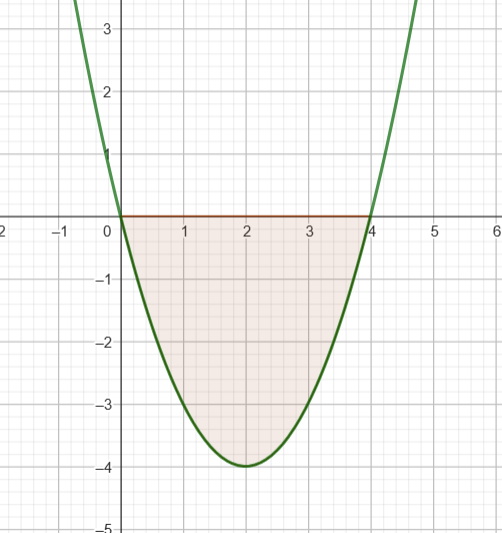
\includegraphics[width=8cm]{Opgave_51-56/Opgave_55/55.png}

Vi kan se at området funktionen $f(x)$ afgrænser med x-aksen ligger mellem x værdierne $x = 0$ og $x = 4$ og er det farvede areal.

Vi beregner nu arealet hvor $a = 0$ og $b = 4$

\begin{align*}
    \int_0^4 x^2 - 4x dx &= \left[\frac{1}{2 + 1}x^{2 + 1} - \frac{4}{1 + 1}x^{1+1} \right]_0^4 = \left[0,33x^3 - 2x^2\right]\\
    &= (0,33\cdot 4^3 - 2\cdot 4^2) - (0,33 \cdot 0^3 - 2 \cdot 0^2)\\
    &= -10,88
\end{align*}

Da vi ikke kan have et negativt areal fjerner vi fortegnet og får arealet $10,88$. 



